\documentclass[11pt,1column]{article}
\usepackage[top=1.5cm, bottom=2.5cm, left=2cm, right=2cm]{geometry}
\usepackage{hyperref}
\usepackage{url}
\usepackage{wrapfig}
\usepackage{setspace}
\usepackage{graphicx,cite,caption,subcaption,comment,xspace,tabularx,multirow}
\usepackage{amsfonts,amssymb}
\usepackage{amsmath,algorithm,amsthm,algpseudocode}
\usepackage[usenames,dvipsnames,svgnames,table]{xcolor}
\usepackage{tikz,tikz-3dplot}
\usepackage{mdframed}
\usetikzlibrary{pgfplots.groupplots}
\usetikzlibrary{patterns}
\usetikzlibrary{shapes.geometric,positioning}
\usetikzlibrary{fit,calc,positioning,decorations.pathreplacing,matrix,decorations.markings,shapes,spy}
\usetikzlibrary{arrows, positioning,decorations.markings, calc,matrix,shadows,fadings,shapes.arrows,patterns,snakes}
\usepackage{xifthen}
\tikzstyle{line}=[draw]
\tikzstyle{arrow}=[draw, -latex] 
\usetikzlibrary{3d}
\usepackage{appendix}
%\usepackage[usenames,dvipsnames]{color}
%\usepackage{fullpage}
%\usepackage{amssymb}
%\usepackage{amsthm}
%\usepackage{hyperref}
\usepackage{pgfplots}
\usepgfplotslibrary{patchplots}
\usepgfplotslibrary{colormaps,external}

\renewcommand{\algorithmicrequire}{\textbf{Input:}}
\renewcommand{\algorithmicensure}{\textbf{Output:}}
\definecolor{shadecolor}{rgb}{1,0.8,0.3}
\newlength{\mylen}
\addtolength{\mylen}{\baselineskip}
\addtolength{\mylen}{9pt}



\newenvironment{bottompar}{\par\vspace*{\fill}}{\clearpage}

\begin{document}

\title{Increase in the Amount of $\hbox{CO}_2$ and Ocean Heat Content}
\author{Wilfred Bony}


\date{}
\maketitle

\begin{center}
Laboratory of AudioVisual Communications (LCAV)\\
Ecole Polytechnique Federale de Lausanne (EPFL)
\end{center}


\section{Summary}
After a week spent meticulously agreeing the exact wording, the Intergovernmental Panel on Climate Change (IPCC) has just released a summary of the first part of its major report reviewing the science of climate change.

\section{The earth’s surface is warming}
Known as the Summary for Policymakers (SPM), the document describes the physical science behind climate change – whittling down the latest findings about how and why earth’s climate is changing to just 36 pages.

It also makes predictions about how temperatures and sea levels might change in the future – relative to their average levels between 1986 and 2005. The two main ones we’ll touch on here are RCP2.6, a low emissions scenario where carbon emissions are rapidly cut, and RCP8.5, a high emissions scenario with no carbon cuts.

But who can be bothered to read a 36 page document? So here are 6 pictures to give you the gist


\section{The amount of carbon dioxide in the atmosphere is rising}
THE record of atmospheric carbon-dioxide levels started by the late Dave Keeling of the Scripps Institution of Oceanography is one of the most crucial of the data sets dealing with global warming. When the measurements started in 1959 the annual average level was 315 parts per million, and it has gone up every year since. To begin with it went up by roughly one part per million per year. Now it is more like two parts per million per year. The figure for 2011 is 391.6. More carbon dioxide in the atmosphere means a stronger greenhouse effect, and various measurements speak to this. Global surface temperature records show a warming over the same period, though because of fluctuations in the climate, air pollution, volcanic eruptions and other confounding factors the rise is nothing like as smooth. A steadier rise can be seen in the heat content of the oceans, measured in terms of the energy stored, rather than the temperature.

\begin{figure}[H]
\begin{center}
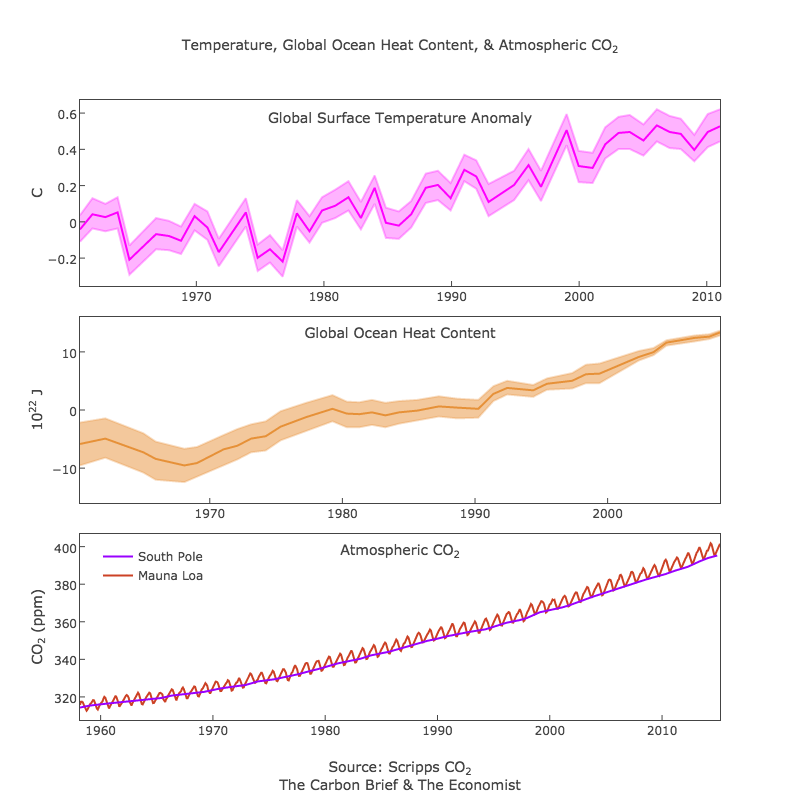
\includegraphics[width=\textwidth]{./Figures/AtmosphericCO2.png}
\caption{$\hbox{CO}_2$ levels and oceans' heat content}
\label{fig:CO2_heat}
\end{center}
\end{figure}


\begin{thebibliography}{00}
\bibitem{Climate_ref}  \emph{Climate changes}, The Economist Online, May 2012,  \url{http://www.economist.com/blogs/graphicdetail/2012/05/daily-chart-1}.
\end{thebibliography}


\end{document}







​